\documentclass[a4paper]{article}
\usepackage[utf8]{inputenc}
\usepackage[T2A]{fontenc}
\usepackage[english, russian]{babel}
\usepackage[left=25mm, top=20mm, right=25mm, bottom=30mm, nohead, nofoot]{geometry}
\usepackage{amsmath, amsfonts, amssymb} % математический пакет
\usepackage {fancybox, fancyhdr}
\usepackage{python}
\pagestyle{fancy}
\fancyhf{}
\fancyhead[R]{Винер Даниил. БЭАД232}
\fancyfoot [R] {\thepage}
\setlength{\footskip}{12.0pt}
% \setlength{\headheight}{12.0pt}
\fancyhead[L]{АиСД. ЭАД ФКН—ФЭН ВШЭ}
\setcounter {page}{1}
\headsep=10mm
\usepackage{xcolor}
\usepackage{cancel}
\usepackage{ulem}
\usepackage{hyperref}
\usepackage{epigraph}
\hypersetup{colorlinks=true, allcolors= [RGB]{010 090 200}} % цвет ссылок
\usepackage {setspace}
\usepackage[pdftex]{graphicx}
\usepackage{ dsfont }
\usepackage{array}
\setcounter{MaxMatrixCols}{20}
\usepackage{mathbbol}
\usepackage{minted}
\usepackage{enumerate}
\usepackage{listings}
\usepackage{indentfirst}
\usepackage{color}
\definecolor{dkgreen}{rgb}{0,0.6,0}
\definecolor{gray}{rgb}{0.5,0.5,0.5}
\definecolor{mauve}{rgb}{0.58,0,0.82}
\lstset{frame=tb,
  language=C++,
  aboveskip=3mm,
  belowskip=3mm,
  showstringspaces=false,
  columns=flexible,
  basicstyle={\small\ttfamily},
  numbers=none,
  numberstyle=\tiny\color{gray},
  keywordstyle=\color{blue},
  commentstyle=\color{dkgreen},
  stringstyle=\color{mauve},
  breaklines=true,
  breakatwhitespace=true,
  tabsize=3
}
% «»

\DeclareRobustCommand{\divby}{%
  \mathrel{\text{\vbox{\baselineskip.65ex\lineskiplimit0pt\hbox{.}\hbox{.}\hbox{.}}}}%
}
\DeclareSymbolFontAlphabet{\mathbb}{AMSb}
\DeclareSymbolFontAlphabet{\mathbbl}{bbold}
\newcommand{\e}{\mathbbl{e}}
\newcommand{\dfs}{\textbf{DFS }}
\definecolor{codegray}{gray}{0.9}
\newcommand{\code}[1]{\colorbox{codegray}{\texttt{#1}}}
\begin{document}
\section*{\LARGE{Алгоритмы и структуры данных. Коллоквиум}}
\begin{flushright}
    \textit{Основано на лекциях и тренировках}\\ 
    \textit{по алгоритмам Михаила Густокашина}
\end{flushright}
\tableofcontents
\newpage
\section{Способы задания графов}
\subsection{Матрица смежности}
\textbf{Матрица смежности} — матрица графа $G=(V,E)$ размера $V\times V$, такая что на пересечении $i-$ой строки и $j-$ого столбца стоит 1, если есть ребро между вершинами $i$ и $j$, и 0 — если иначе\\[2mm]
\indent\textbf{Сложность построения} — $O(V^2)$

\subsection{Список смежности}
\textbf{Список смежности} — массив, в котором каждой вершине графа соответствует список, состоящий из соседей этой вершины\\[2mm]
\indent Изначально создается $V$ динамически расширяемых пустых векторов\\[2mm]
\indent При считывании ребра $A_i-B_i$ в вектор с номером $A_i$ добавляется ребро $B_i$ (если граф неориентированый, то еще в вектор с номером $B_i$ добавляется ребро $A_i$)\\[2mm]
\indent\textbf{Сложность построения} — $O(E)$\\[2mm]
\indent\textbf{Сложность нахождения всех соседей каждой вершины} — $O(V+E)$, так как мы проходим по всем вершинам за $V$ и просматриваем каждое ребро за $E$

\subsection{Список ребер}
\textbf{Список ребер} — структура данных, представляющая собой набор из пар $A_i-B_i$, где $A_i,B_i$ — вершины графа\\[2mm]
\indentПорядок в списке ребер не важен \textbf{только в случае неориентированных} графов
\subsubsection*{Сложность нахождения всех соседей каждой вершины}
Если граф неориентирован, то оптимально будет сделать его ориентированным (помимо ребра $A_i-B_i$ добавить ребро $B_i-A_i$)\\[2mm]
\indent Сортировка ребер — $O(E\log E)$; поиск первого соседа в списке ребер для одной вершины — $O(\log E)$, для двух — $O(V\log E)$\\[2mm]
Так как обычно в графах $E\geqslant V$, то для поиска всех соседей всех вершин потребуется $O(E\log E)$





\section{Обход в глубину}
\subsection{Обход в глубину}
\subsubsection*{Описание алгоритма}
Обход начинается с любой вершины графа. Из этой вершины мы переходим в одного из непосещенных соседей. Если все соседи посещены, то мы возвращаемся вдоль всего пройденного пути, пока не наткнемся на вершину, у которой есть непосещенный сосед. Алгоритм завершает работу, когда мы возвращаемся в исходную вершину и все ее соседи посещены
\subsubsection*{Применение алгоритма}
\begin{enumerate}
    \item Поиск случайного пути в лабиринте
    \item Решение задач, связанных с построением маршрута: в сети, на карте, в сервисах покупки билетов и так далее
    \item Поиск циклов, сортировки
\end{enumerate}
\subsubsection*{Асимптотика}
\label{dfs_asimp}
Сложность зависит от представления графа: матрица смежности, список ребер или список смежности\\[2mm]
\indent Рассмотрим каждый вариант:
\begin{enumerate}
    \item Список смежности — $O(V+E)$
    \begin{itemize}
        \item Вершины посещаются (проверяются на посещенность) только один раз, что составляет $O(V)$
        \item Каждое ребро проверяется ровно один раз, что составляет $O(E)$
    \end{itemize}
    \item Матрица смежности — $O(V^2)$
    \begin{itemize}
        \item Вся матрица имеет размер $V\times V$
        % \item Для каждой вершины проверяется все возможные $V$ соседей, даже если они не сосединены ребром
    \end{itemize}
\end{enumerate}
\subsubsection*{Пример}
\begin{center}
    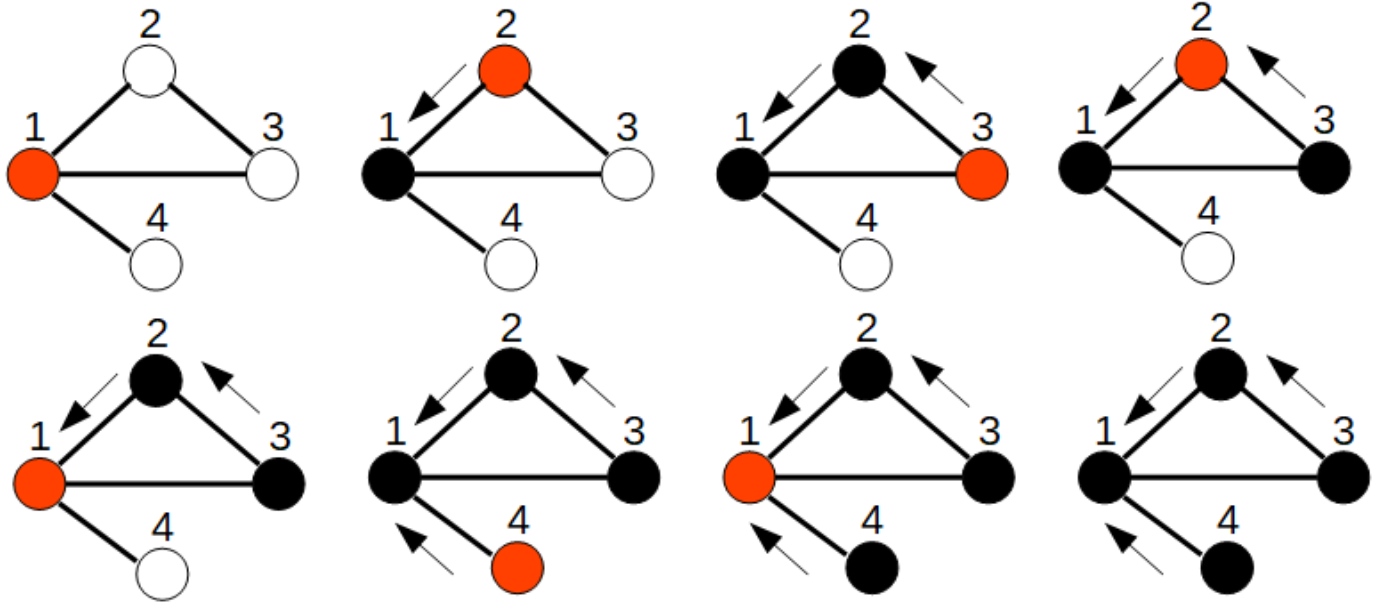
\includegraphics[width=0.8\linewidth]{dfs.png}
    \label{dfs}
\end{center}
\subsubsection*{Псевдокод}
\begin{lstlisting}
void dfs(int v){
    used[v] = 1;
    for (auto to : gr[v]){
        if (!used[to]){
            dfs(to);
        }
    }
}
\end{lstlisting}

\subsection{Связность}
\textbf{Связный граф} — граф, в котором существует путь от любой вершины до любой другой вершины
\subsubsection*{Проверка графа на связность}
\begin{enumerate}
    \item Запуск DFS от каждой из вершин графа
    \begin{itemize}
        \item Для каждого из обходов необходимо проверить, что посещены все вершины
        \item Сложность составит $O(V\times E)$
    \end{itemize}
    \item Запуск DFS от любой вершины
    \begin{itemize}
        \item Если от вершины 1 в неориентированном графе можно попасть в $v$ и в $u$, то существует путь от $v$ до $u$
        \item Так как есть путь из 1 в $v$, то в неориентированном графе существует и обратный путь из $v$ в 1, а оттуда можно попасть в $u$
        \item Сложность такого подхода зависит от сложности DFS — \ref{dfs_asimp}
    \end{itemize}
\end{enumerate}

\subsection{Поиск компонент связности в графе}
\label{2.3}
\textbf{Компонента связности графа} — подмножество вершин и соединяющих их ребер, такое что есть путь путь из каждой вершины в каждую
\subsubsection*{Алгоритм поиска компоненты связности}
Можно раскрасить граф в компоненты связности. Каждой вершине ставится в соответствие номер компоненты связности, к которой относится вершина\\[2mm]
\indent \textbf{Реализация происходит через DFS}\\
Может потребоваться несколько запусков поиска в глубину. Поэтому поиск проводим через цикл, перебирающий все вершины
\begin{itemize}
    \item Заводим массив длинной $V$ для хранения цвета каждой вершины
    \item При входе в DFS красим вершину в текущий цвет
    \item Если очередная вершина не покрашена, то счетчик количества компонент связности увеличивается и запускается DFS для этой вершины со значением цвета равным текущему значению счетчика
\end{itemize}

\subsection{Поиск цикла в графе}
Чтобы найти цикл в графе нужно раскрасить его в три цвета:
\begin{itemize}
    \item \textbf{Белый} — вершина непосещенная
    \item \textbf{Серый} — DFS вошел в вершину, но не обработал всех соседей
    \item \textbf{Черный} — Все соседи вершины посещены и помечены черным
\end{itemize}
$$\boxed{\text{Если в графе есть обратные ребра, т.е. ребра ведущие в серую вершину, то в графе есть цикл}}$$
\subsubsection*{Алгоритм}
\begin{itemize}
    \item В каждый момент времени серым цветом будут помечены вершины, лежащие на пути \dfs от стартовой вершины до текущей
    \item Если из текущей вершины $u$ есть ребро в серую вершину $v$, то в графе есть цикл, т.к. существует путь от $v$ до $u$ ($v$ лежит на пути от стартовой вершины до $u$) и путь от $u$ до $v$, проходящий по одному ребру
\end{itemize}
\subsubsection*{Восстановление цикла}
Допустим, для $u$ нашелся серый сосед $v$, тогда запоминаем номер $v$ и выходим из рекурсивной функции, запоминая номера вершин, пока не дойдем до вершины, в которой нашелся цикл 
 
\subsection{Проверка графа на двудольность}
\textit{Примечание.} Граф — двудольный тогда и только тогда, когда все циклы в графе имеют четную длину\\[2mm]
\textbf{Алгоритм}
\begin{itemize}
    \item Выбираем произвольную вершину и красим ее в цвет \textit{color}
    \item Всех соседей этой вершины красим в цвет $3-color$
    \item Соседей соседей — в цвет \textit{color} и т.д.
    \item Если в какой-то момент сосед вершины уже покрашен в тот же цвет, что и вершина, то алгоритм завершает работу, так как граф не двудольный, потому что есть циклы нечетной длины
\end{itemize}
Если граф не является связным, то нужно запустить \dfs из каждой вершины каждой компоненты связности (как в п. \ref{2.3})


\subsection{Диаметр и центр дерева}
\textbf{Диаметр дерева} — максимальная длина (в рёбрах) кратчайшего пути в дереве между любыми двумя вершинами\\[2mm]
\indent\textbf{Центр дерева} — вершины (одна или две) максимально удаленные от других вершин дерева\\
\indent\indent\textit{Примечание.} Центр можно понимать так: это вершина дерева, такая что при подвешивании дерева за нее глубина дерева минимальна
\subsubsection*{Алгоритм поиска диаметра дерева}
Требуется использовать два \dfs
\begin{itemize}
    \item Берем любую вершину дерева (пусть это $a$) и ищем самую удаленную от нее вершину $b$ с помощью \dfs
    \item Из вершины $b$ запускаем \dfs и ищем самую удаленную от нее вершину (пусть это $c$)
    \item Путь из $b$ в $c$ — диаметр дерева
\end{itemize}

\begin{lstlisting}
    std::vector<node> find_diameter() {
        std::vector<node> ans, path;
        std::vector<int> used(gr_.size(), 0);

        std::function<void(node v)> dfs = [&] (node v) {
            used[v] = true;
            path.emplace_back(v);
            for (const auto& to : gr_[v]) {
                if (!used[to]) {
                    dfs(to);
                }
            }
            if (ans.size() < path.size()) {
                ans = path;
            }
            path.pop_back();
        };
        dfs(0);
        used.assign(gr_.size(), 0);
        dfs(ans.back());
        return ans;
    }
\end{lstlisting}

\section{Задача построения дерева кратчайших расстояний}
\subsection{Обход в ширину}
\subsubsection*{Наивный алгоритм}
Создаем массив, заполняем его бесконечностью ($v+1$, например). Для начальной вершины установим значение 0\\[2mm]
\indent Выполняем $v-1$ шагов. Нужно перебрать все вершины и выбрать те, которые находятся на расстоянии равном номеру шага, а также пометить все соседние вершины числом на 1 большим, чем номер текущего шага
\begin{itemize}
    \item На нулевом шаге выбираем начальную вершину и помечаем ее соседей 1
    \item Затем выбираем вершины, находящиеся на расстоянии 1 и их непомечанных соседей помечаем 2 и т.д.
\end{itemize}
\indent \textbf{Сложность} — $O(V^2+E)$, так как мы сделаем $V$ шагов, переберем $V$ вершин, а также просмотрим все ребра
\subsubsection*{Реализация через очередь}
В начале очереди находятся вершины текущего шага, а в конце — следующего
\begin{itemize}
    \item Помещаем начальную вершину в очередь, а в масив расстояний ставим 0 для нее
    \item Берем первый (верхний) элемент из очереди и просматриваем соседей
    \item Если сосед не посещался, то добавляем его в очередь, помечаем вершину как посещенную
    \item Если сосед является пунктом назначения, алгоритм завершает работу
\end{itemize}
\indent\textbf{Время работы} — $O(V+E)$
\subsubsection*{Применение алгоритма}
\begin{enumerate}
    \item Для поиска кратчайшего пути в неявно заданных и невзвешенных графах
    \item Для обнаружения кратчайших путей и минимальных покрывающих деревьев
    % \item Для построения индексов веб-страниц
\end{enumerate}
\indent \textit{Белый} — еще не посещенные вершины, \textit{черный} — уже посещенный, \textit{красный} — обрабатывающиеся в данный момент (в начале очереди), \textit{серый} — вершины, находящиеся в очереди
\begin{center}
    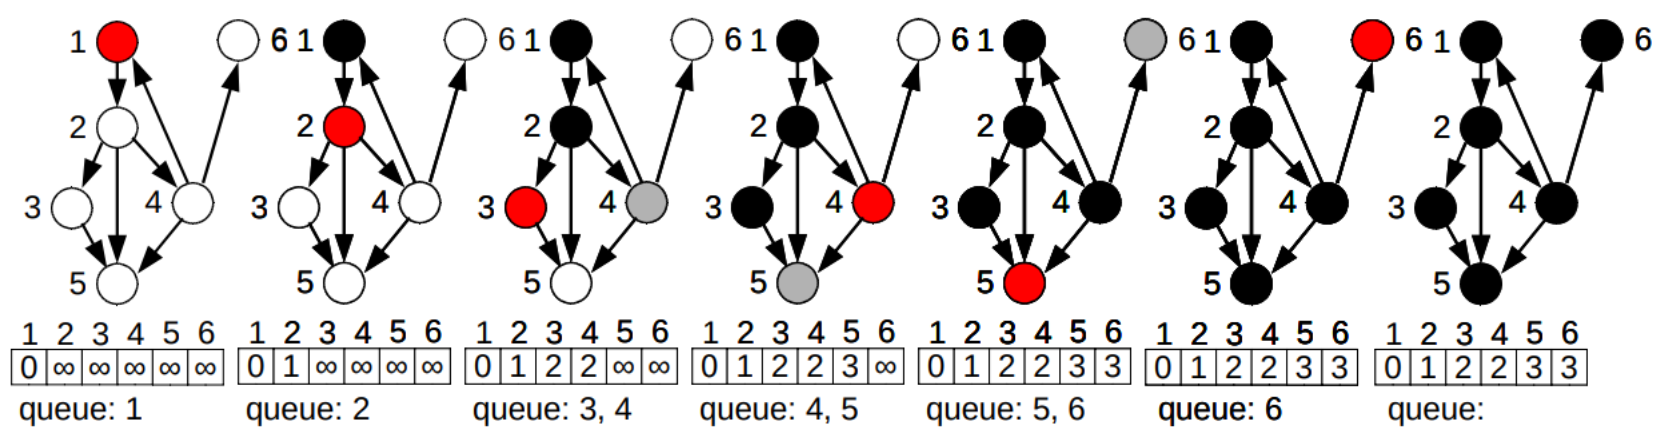
\includegraphics[width=1\linewidth]{bfs.png}
    \label{bfs}
\end{center}

\subsection{Алгоритм Дейкстры}
\subsection*{Случай для плотного графа}
Создадим такие массивы
\begin{itemize}
    \item \code{dist} — размером $v+1$. В нем для каждой вершины хранится текущая длина кратчайшего пути от начальной вершины $s$. (\code{d[s] = 0}, а все остальное — inf)
    \item \code{visited} — размером $v+1$. Хранит иформацию о том, обработана вершина или нет
\end{itemize}
Алгоритм состоит из $v-1$ шага. На каждом шаге делаем следующее
\begin{enumerate}
    \item Выбираем необработанную вершину $v$ с минимальным расстоянием от начальной вершины. Помечаем $v$ как обработанную
    \item Производим релаксацию: рассматриваем все вершины, соседние с $v$ (вес ребра $(u,v)=w$) и для соседней вершины $u$ пытаемся улучшить значение \textbf{dist[u]}, т.е. \textbf{dist[u]=min(dist[u], dist[v]+w)}
\end{enumerate}
% \textit{Красный} — вершины, для которых будет произведена релаксация, \textit{серый} — обработанные вершины\\
\begin{center}
    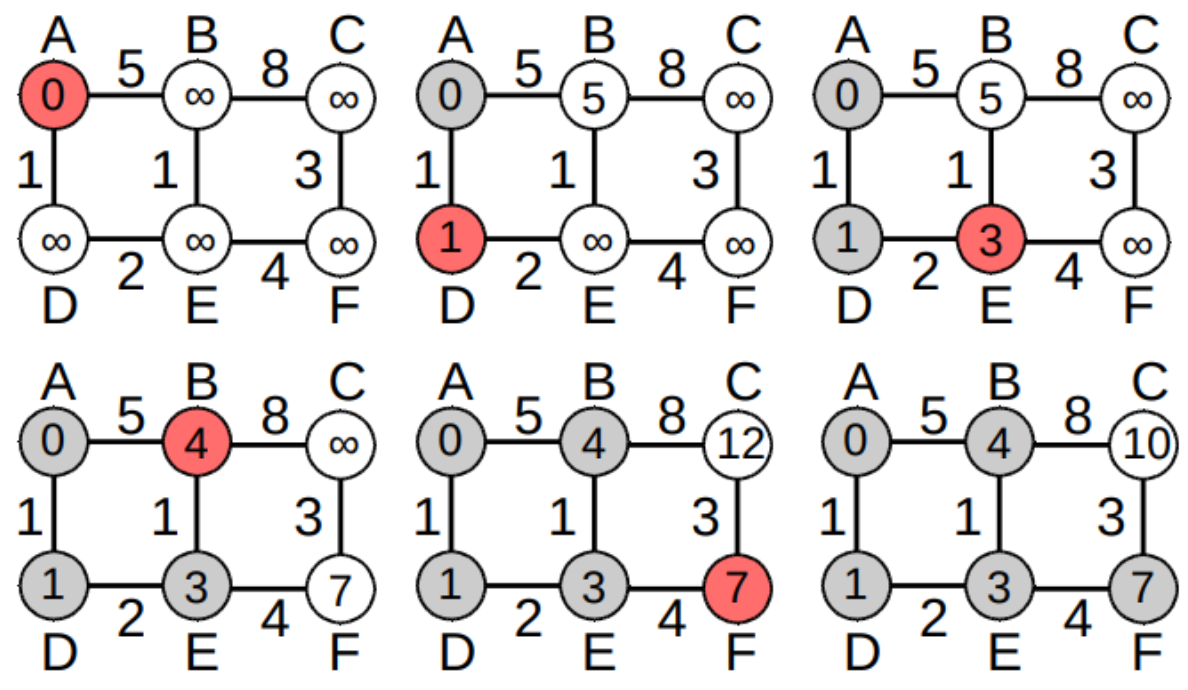
\includegraphics[width=0.8\linewidth]{dijkstra.png}
    \label{dijkstra}
\end{center}
\textit{Красный} — вершины, для которых будет произведена релаксация, \textit{серый} — обработанные вершины\\[2mm]
\textbf{Сложность со списком смежности} — $O(V^2+E)$, так как мы на каждом из $v-1$ шагов ищем минимум из $V$ чисел для вершин и просматриваем каждое ребро один раз\\[2mm]
\textbf{Сложность с матрицей смежности} — $O(V^2)$
\subsection*{Случай для разряженного графа}
\indent \textit{Reminder.} Разряженным назвается граф, у которого количество ребер значительно меньше, чем $V^2$ \\[2mm]
Алгоритм Дейкстры для разреженных графов работает следующим образом:
\begin{enumerate}
    \item Инициализация:
    \begin{itemize}
        \item Задаётся начальная вершина, от которой будут рассчитываться кратчайшие пути
        \item Все расстояния до остальных вершин инициализируются как бесконечность, кроме начальной вершины, для которой расстояние равно нулю
        \item Создаётся структура данных, например, \code{ordered set} или куча, для хранения и быстрого доступа к вершинам и их текущим кратчайшим расстояниям
    \end{itemize}
    \item Пока есть непосещённые вершины:
    \begin{itemize}
        \item Выбирается вершина с минимальным текущим расстоянием (с использованием кучи или \code{ordered set})
        \item Эта вершина помечается как посещённая
        \item Для каждой соседней вершины, смежной с текущей:
        \begin{itemize}
            \item Рассчитывается новое потенциальное расстояние как сумма текущего расстояния до рассматриваемой вершины и веса ребра между текущей вершиной и соседней
            \item Если новое расстояние меньше известного расстояния до соседней вершины:
            \begin{itemize}
                \item Обновляется расстояние до соседней вершины
                \item В \code{ordered set} или куче обновляется информация о расстоянии до этой вершины
            \end{itemize}
        \end{itemize}
    \end{itemize}
    \item Обновление структуры данных:
    \begin{itemize}
        \item При обновлении расстояний до соседних вершин, в структуре данных (куче или \code{ordered set}) происходит операция удаления старого значения и добавления нового значения, что обеспечивает эффективность алгоритма
        \item В случае использования кучи без изменения элементов (например, \code{priority queue}) просто добавляются новые значения, а устаревшие игнорируются
    \end{itemize}
\end{enumerate}
\indent Процесс повторяется, пока не будут посещены все вершины или не будут определены кратчайшие пути до всех достижимых вершин\\[2mm]
\indent \textbf{Сложность —} $O(E\log{V} + V\log{V})$. Узнаем минимум за $O(1)$ (удаление минимума тратит $O(\log{V})$), изменяем элементы за $O(\log{V})$. Для большинства графов сложность будет просто $O(E\log{V})$, так как каждое из $E$ ребер может привести к уменьшению пути и изменению значения в set\\[2mm]
\indent В итоге массив расстояний содержит кратчайшие пути от начальной вершины до всех остальных вершин


\subsection{Алгоритм Форда-Беллмана}
Создадим такой массив
\begin{itemize}
    \item \code{dist} — размером $v+1$. Массив кратчайших расстояний. (\code{d[s] = 0}, а все остальное — inf)
\end{itemize}
Алгоритм состоит из $v-1$ шага. Пусть есть ребро $(u,v)$ и его вес $w$. На каждом шаге перебираем все ребра и проводим релаксацию по этому ребру, то есть
\begin{lstlisting}
    if (dist[v] > dist[u] + w && dist[v] != inf){
        dist[v] = dist[u] + w
    }
\end{lstlisting}
\subsubsection*{Применение алгоритма}
Алгоритм хорош в поиске кратчайших путей от одной вершины до всех остальных на разряженных графах, если в графе есть отрицательные ребра\\[2mm]
\textbf{Сложность} — $O(V\times E)$

\subsection{Алгоритм Левита}
Пусть $d_i$ — текущая длина кратчайшего пути до вершины $i$. Изначально, все элементы $d$, кроме $s$-го равны бесконечности, \code{d[s] = 0}\\[2mm]
\indentРазделим вершины на три множества:
\begin{itemize}
    \item $M_0$ — вершины, расстояние до которых уже вычислено (возможно, не окончательно),
    \item $M_1$ — вершины, расстояние до которых вычисляется. Это множество в свою очередь делится на две очереди:
    \begin{enumerate}
        \item $M_1'$ — основная очередь,
        \item $M_1''$ — срочная очередь;
    \end{enumerate}
    \item $M_2$ — вершины, расстояние до которых еще не вычислено.
\end{itemize}
Изначально все вершины, кроме $s$ помещаются в множество $M_2$. Вершина $s$ помещается в множество $M_1$ (в любую из очередей)\\[2mm]
\indent\textbf{Работа алгоритма:} выбирается вершина $u$ из $M_1$. Если очередь $M_1''$ не пуста, то вершина берется из нее, иначе из $M_1'$. Для каждого ребра $(u,v)$ и весом $w$ возможны три случая:
\begin{itemize}
    \item $v \in M_2$, то $v$ переводится в конец очереди $M_1'$. И производится релаксация ребра $(u,v)$: \code{d[v]= d[u] + w},
    \item $v \in M_1$, то происходит релаксация ребра $(u,v)$,
    \item $v \in M_0$. Если при этом \code{d[v] > d[u] + w}, то происходит релаксация ребра $(u,v)$ и вершина $v$ помещается в $M_1''$; иначе ничего не делаем
\end{itemize}
В конце шага помещаем вершину $u$ в множество $M_0$\\[2mm]
Алгоритм заканчивает работу, когда множество $M_1$ становится пустым\\[2mm]
\indent\textbf{Сложность} — $O(V^2E)$, так как при обработке каждой вершины приходится обрабатывать $n-1$ ребро

\subsection{Алгоритм Флойда}
Работаем с матрицей смежности, которую будем превращать в матрицу кратчайших расстояний\\[2mm]
\indent Алгоритм пройдет $V$ шагов. Перед $k$-м шагом на позиции \code{dist[from][to]} стоит длина кратчайшего пути из from в to, проходящего только через промежуточные вершины с номерами, меньше $k$\\[2mm]
\indent На первом шаге матрица смежности равна матрице \code{dist}, а отсутствующие ребра помечены как inf\\[2mm]
\indent При переходе от $k-1$ шага к $k$ нужно пересчитать матрицу расстояний, т.е. добавить в нее кратчайшие пути, проходящие через $k$. При пересчете пути из from в to возможны случаи:
\begin{enumerate}
    \item Кратчайший путь из from в to не проходит через $k$, поэтому мы его не меняем
    \item Кратчайший путь из from в to проходит через $k$: делим этот путь на две части — от from до $k$ и от $k$ до to. Тогда длина нового пути равна \code{dist[from][k] + dist[k][to]}
\end{enumerate}
\subsubsection*{Применение алгоритма}
Алгоритм прменяется в задаче поиска кратчайших путей от каждой вершины до каждой. Его использование проще в написании, чем алгоритм Дейкстры\\[2mm]
\indent\textbf{Сложность} — $O(V^3)$, т.е. перебор всевозможных from и to\\[2mm]
\indent\textbf{Требуется памяти} — $V^3$, однако, если хранить две матрицы, тогда требуемая память сократиться до $V^2$
% \subsubsection*{Реализация}
% \begin{lstlisting}
%     for (size_t k = 1; k <= v; ++k){
%         for (size_t from = 1; from <= v; ++from){
%             for (size_t to = 1; to <= v; ++to){
%                 dist[from][to] = min(dist[from][to], dist[from][k] + dist[k][to])
%             }
%         }
%     }
% \end{lstlisting}

\section{Задача union — find}
\subsection{Задача union — find}
Пусть у нас есть $N$ элементов, занумерованных от 1 до $N$. Изначально каждый элемент находится в своем отдельном множестве (также занумерованных от 1 до $N$). Нам необходимо поддерживать такие опреации:
\begin{itemize}
    \item \code{find(x)} — найти номер множетсва, в котором лежит $x$
    \item \code{union(x, y)} — объединить множества, содержащие $x$ и $y$
    \item Можно добавить, но необязательно:
    \begin{itemize}
        \item \code{make(x)} — создает новое множество, содержащее $x$ 
    \end{itemize}
\end{itemize}
\begin{center}
    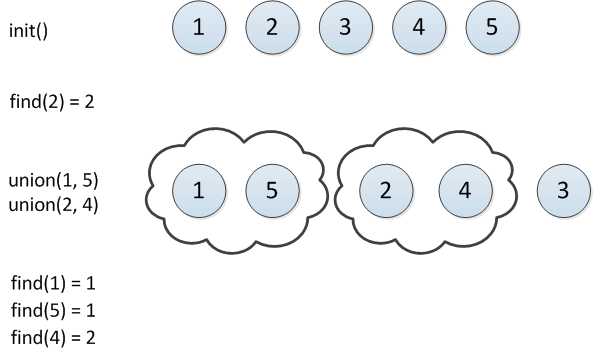
\includegraphics[width=0.6\linewidth]{DSU_1_Example.png}
    \label{union-find}
\end{center}

\subsection{Наивная реализация}
\begin{enumerate}
    \item Создаем массив с индексами от 1 до $N$
    \begin{itemize}
        \item Индекс означает номер элемента
        \item Значение по индексу — номер множества, к которому относится элемент
    \end{itemize}
    \item Операция \code{find(x)}
    \begin{itemize}
        \item Нужно вернуть содержимое ячейки с номером $x$
        \item \textbf{Сложность} — $O(1)$
    \end{itemize}
    \item Операция \code{union(x, y)}
    \begin{itemize}
        \item Узнаем номера множеств, содеражащих эти элементы (пусть это $a$ и $b$ соответственно)
        \item Проходим по всему массиву и заменяем значения $b$ на $a$
        \item \textbf{Сложность одной операции} — $O(N)$
        \item \textbf{Сложность объединения всех множеств} — $O(N^2)$
    \end{itemize}
\end{enumerate}

\subsection{Реализация с использованием линейных списков}
Идея этой реализации заключается в том, что мы заводим второй масиив, на индексах которого стоят номера множеств, а по индексу хранится список элементов соответствующего множества\\[2mm]
\indent Тогда при вызове \code{union(x, y)} мы делаем так: \code{max(x, y) += min(x, y)}
\subsubsection*{Сложность}
Так как мы храним второй масиив, то мы \textit{теряем в памяти}, однако алгоритм будет работать \textit{быстрее}, за $O(N\log N)$, так как делаем $O(\log N)$ шагов на кажом шаге $O(N)$ для объединения множеств
\begin{center}
    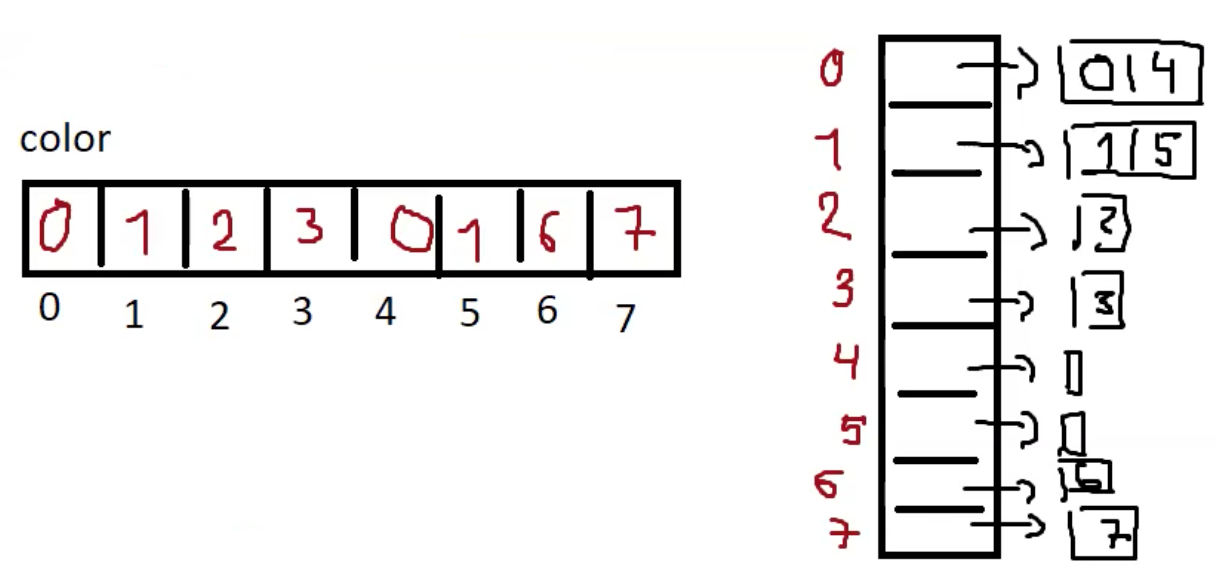
\includegraphics[width=0.75\linewidth]{linlist2.png}
    \label{union-find-lin}
\end{center}

\subsection{Система непересекающихся множеств}
Идея заключается в хранении каждого множества в виде дерева\\[2mm]
\indent Мы имеем один единственный массив предков \code{p}. Индексы в нем — номера элементов, а по индексу хранится номер предка
\begin{center}
    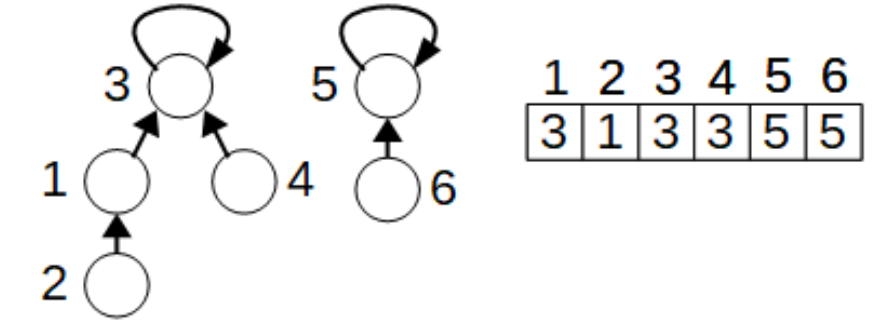
\includegraphics[width=0.6\linewidth]{snm.png}
    \label{dsu}
\end{center}
В данном примере, петли означают, что это корень дерева, а в \code{p} на позицию с номером корня записывается значение самого корня\\[2mm]
Вместо этого, в \code{p} на позицию корня можно поставить $-1$, суть не изменится\\[2mm]
Тогда операции \code{find(x)} и \code{union(x, y)} можно реализовать так:
\begin{lstlisting}
    int find(x){
        while (p[v] != -1){
            v = p[v]
        }
        return v
    }
    
    void union(x, y){
        p[find(x)] = find(y)
    }
\end{lstlisting}
\indent\textbf{Сложность} — $O(N^2)$
\subsubsection{Сжатие путей}
Идея заключается в том, что когда мы найдём искомого предка $p$ множества (с помощью \code{find(x)}), то запомним, что у вершины $x$ и всех пройденных по пути вершин — именно этот предок $p$. Проще всего это сделать, перенаправив их {\rm parent}[] на эту вершину $p$\\[2mm]
\indent Теперь в массиве предков для каждой вершины там может храниться не непосредственный предок, а предок предка, предок предка предка, и т.д\\[2mm]
\indent \textbf{Сложность} — $O(\log N)$

\subsubsection{Объединение деревьев}
Идея: нужно подвешивать дерево с большей глубиной к дереву с меньшей глубиной\\[2mm]
\indent Для каждого дерева храним его глубину в массиве\\[2mm]
\indent \textbf{Сложность} — $O(\log N)$

\subsection{Алгоритм Краскала}
\begin{itemize}
    \item Отсортируем все ребра по возрастанию
    \item Каждая вершина находится в своем отдельном множестве
    \item В остовное дерево берем те ребра, которые соединяют разные множества вершин
    \item При добавлении ребра происходит объединение множеств
\end{itemize}
Алгоритм используется для построения минимального остовного дерева в графе

\section{Дерево поиска}
\textbf{\textit{Бинарное дерево поиска}} — дерево, для которого выполняются следующие свойства:
\begin{itemize}
\item У каждой вершины не более двух детей
\item Все вершины обладают \textit{ключами}, на которых определена операция сравнения (например, целые числа или строки)
\item У всех вершин \textit{левого} поддерева вершины $v$ ключи \textit{не больше}, чем ключ $v$
\item У всех вершин \textit{правого} поддерева вершины $v$ ключи \textit{больше}, чем ключ $v$
\item Оба поддерева — левое и правое — являются двоичными деревьями поиска
\end{itemize}
В \textit{небинарных} (\sout{нетрадиционных}) деревьях количество детей может быть больше двух, и при этом в «более левых» поддеревьях ключи должны быть меньше, чем «более правых»\\[2mm]
\indent Для работы с деревьями поиска нужно создать структуру
\begin{lstlisting}
struct Node:
  T key                    // key of the node
  Node left                // pointer to the left child
  Node right               // pointer to the right child
  Node parent              // pointer to the parent
\end{lstlisting}
\subsection{Поиск элемента}
Нужна функция, прнимающая корень дерева и искомый ключ
\begin{itemize}
    \item Для каждого узла сравниваем значение его ключа с искомым ключом
    \item Если ключи одинаковы, то функция возвращает текущий узел
    \item В противном случае функция вызывается рекурсивно для левого или правого поддерева
\end{itemize}
\begin{lstlisting}
Node search(x : Node, k : T):
   if x == null or k == x.key
      return x
   if k < x.key
      return search(x.left, k)
   else
      return search(x.right, k)
\end{lstlisting}
\textbf{Сложность в худшем случае} — $O(h)$ ($h$ — высота дерева), так как узлы, которые посещает функция образуют нисходящее дерево. Такое возможно, когда дерево является «бамбуком»\\[2mm]
\textbf{Сложность при оптимизации} — $O(\log N)$. Если изменить способ хранения дерева, например сразу при проходе до какого-то ключа записать его как ключ ко всем вершинам в пути, то сложность снизится

\subsection{Вставка элемента}
Почти то же самое, что поиск элемента, но теперь при обнаружении у элемента отсутствия ребенка нужно подвесить на него вставляемый элемент
\begin{lstlisting}
Node insert(x : Node, z : T):               // x - root of the subtree, z - key to be inserted
   if x == null 
      return Node(z)                        // attach a Node with key = z
   else if z < x.key
      x.left = insert(x.left, z)
   else if z > x.key
      x.right = insert(x.right, z)
   return x
\end{lstlisting}

\subsection{Удаление элемента}
Рассмотрим три случая при рекурсивной реализации
\begin{enumerate}
    \item Удаляемый элемент находится в \textit{левом} поддереве текущего поддерева
    \begin{itemize}
        \item тогда нужно рекурсивно удалить элемент из нужного поддерева
    \end{itemize}
    \item Удаляемый элемент находится в \textit{правом} поддереве
    \begin{itemize}
        \item тогда нужно рекурсивно удалить элемент из нужного поддерева
    \end{itemize}
    \item Удаляемый элемент находится в \textit{корне}, то два случая:
    \begin{itemize}
        \item имеет два дочерних узла
        \begin{itemize}
            \item нужно заменить его минимальным элементом из правого поддерева и рекурсивно удалить этот минимальный элемент из правого поддерева
        \end{itemize}
        \item имеет один дочерний узел
        \begin{itemize}
            \item нужно заменить удаляемый элемент потомком
        \end{itemize}
    \end{itemize}
\end{enumerate}
\begin{lstlisting}
Node delete(root : Node, z : T):    // root of subtree, key to delete
  if root == null
    return root
  if z < root.key
    root.left = delete(root.left, z)
  else if z > root.key
    root.right = delete(root.right, z)
  else if root.left != null and root.right != null
    root.key = minimum(root.right).key
    root.right = delete(root.right, root.key)
  else
    if root.left != null
      root = root.left
    else if root.right != null
      root = root.right
    else
      root = null
  return root
\end{lstlisting}
% \subsubsection*{Еще один вариант объяснения}
% \begin{enumerate}
%     \item Если пытаемся удалить лист или какую-то вершину в одном из поддеревьев, то все хорошо. Просто вырезаем вершину и на ее место ставим потомка и всех потомков потомка
%     \item Если же пытаемся удалить 
% \end{enumerate}

\section{Дерево отрезков}
\subsection{Дерево отрезков}
Дан массив $a$ из $n$ целых чисел, и требуется отвечать на запросы двух типов:
\begin{enumerate}
    \item Изменить значение в ячейке (т. е. реагировать на присвоение \code{a[k] = x})
    \item Вывести сумму элементов $a_i$ на отрезке с $l$ по $r$
\end{enumerate}
Несколько изменим массив
\begin{itemize}
    \item Посчитаем сумму всего массива и где-нибудь запишем
    \item Разделим его пополам, посчитаем сумму на половинах и тоже где-нибудь запишем
    \item Каждую половину разделим пополам ещё раз, и т.д., пока не придём к отрезкам длины 1
\end{itemize}
\begin{center}
    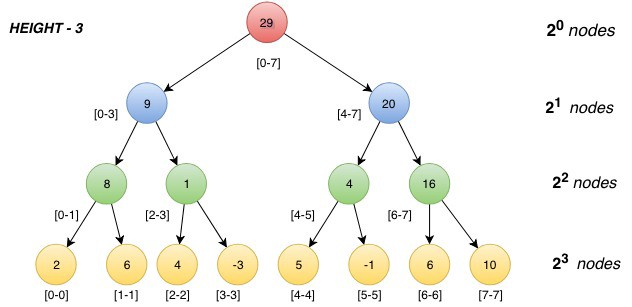
\includegraphics[width=0.9\linewidth]{segtree-example.jpg}
    \label{segtree-ex}
\end{center}
Корень этого дерева соответствует отрезку $[0, n)$, а каждая вершина (не считая листьев) имеет ровно двух сыновей, которые тоже соответствуют каким-то отрезкам

\subsection{Операции на отрезке}
Здесь представлены операции на отрезке, реализованные с помощью указателей. Эта реализация не самая эффективная, но самая простая, решающая большинство задач. Подробнее о других реализациях \href{http://e-maxx.ru/algo/segment_tree}{тут} и \href{https://codeforces.com/blog/entry/18051}{тут}
% \indent Можно ввести нумерацию вершин и расположить их в массиве, подробнее об этом \href{http://e-maxx.ru/algo/segment_tree}{тут} и \href{https://codeforces.com/blog/entry/18051}{тут}
\subsubsection{Построение}
Строить дерево отрезков можно рекурсивным конструктором, который создает детей, пока не доходит до листьев\\[2mm]
\indent Если изначально массив не нулевой, то можно параллельно с проведением ссылок насчитывать суммы\\[2mm]
\indent \textbf{Сложность} — $O(n)$
\begin{lstlisting}
Segtree(int lb, int rb) : lb(lb), rb(rb) {
    if (lb + 1 == rb)
        s = a[lb];
    else {
        int t = (lb + rb) / 2;
        l = new Segtree(lb, t);
        r = new Segtree(t, rb);
        s = l->s + r->s;
    }
}
\end{lstlisting}

\subsubsection{Изменение}
Для запроса прибавления будем рекурсивно спускаться вниз, пока не дойдем до листа, соответствующего элементу $k$, и на всех промежуточных вершинах прибавим $x$:
\begin{lstlisting}
void add(int k, int x) {
    s += x;
    if (l){
        if (k < l->rb)
            l->add(k, x);
        else
            r->add(k, x);
    }
}
\end{lstlisting}
\indent \textbf{Сложность} — $O(\log n)$

\subsubsection{Сумма}
Нужно делать разбор случаев, как отрезок запроса пересекается с отрезком вершины:
\begin{enumerate}
    \item Если лежит полностью в отрезке запроса, вывести сумму
    \item Если не пересекается с отрезком запроса, вывести ноль
    \item else: рекурсивно запускаемся от детей
\end{enumerate}
\begin{lstlisting}
int sum(int lq, int rq) {
    if (lb >= lq && rb <= rq)
        return s;
    if (max(lb, lq) >= min(rb, rq))
        return 0;
    return l->sum(lq, rq) + r->sum(lq, rq);
}
\end{lstlisting}
\indent \textbf{Сложность} — $O(\log n)$. На каждом уровне дерева отрезков, наша рекурсивная функция могла посетить максимум четыре отрезка; тогда, учитывая оценку $O (\log n)$ для высоты дерева, мы получаем асимптотику времени работы алгоритма


\subsection{Применение дерева отрезков}
Дерево отрезков может применяться в таких задачах, как
\begin{itemize}
    \item поиск суммы на подотрезке
    \item поиск минимума/максимума на отрезкее
    \item массовые изменения массивов (например, добавление элемента ко всем элементам сразу)
\end{itemize}


\section{Декартово дерево}
\subsection{По явному ключу}
Имеется бинарное деревео. Каждые его узел (обозначим как ключ $x$) дополняем случайным числом $y$. По ключам $x$ образуется бинарное дерево поиска, а структура, полученная по $y$, обладает свойством двоичной кучи максимумов\\[2mm]
\indent Еще способ:
\begin{itemize}
    \item Нанесём на плоскость набор из $n$ точек. Их $x$ назовем \textit{ключом}, а $y$ \textit{приоритетом}
    \item Выберем самую верхнюю точку (с наибольшим $y$, а если таких несколько — любую) и назовём её \textit{корнем}
    \item От всех вершин, лежащих слева (с меньшим $x$) от корня, рекурсивно запустим этот же процесс. Если слева была хоть одна вершина, то присоединим корень левой части в качестве левого сына текущего корня
    \item Аналогично, запустимся от правой части и добавим корню правого сына
\end{itemize}
% \indent Одно и то же дерево в обычном представлении и в виде декартового дерева:
\begin{center}
    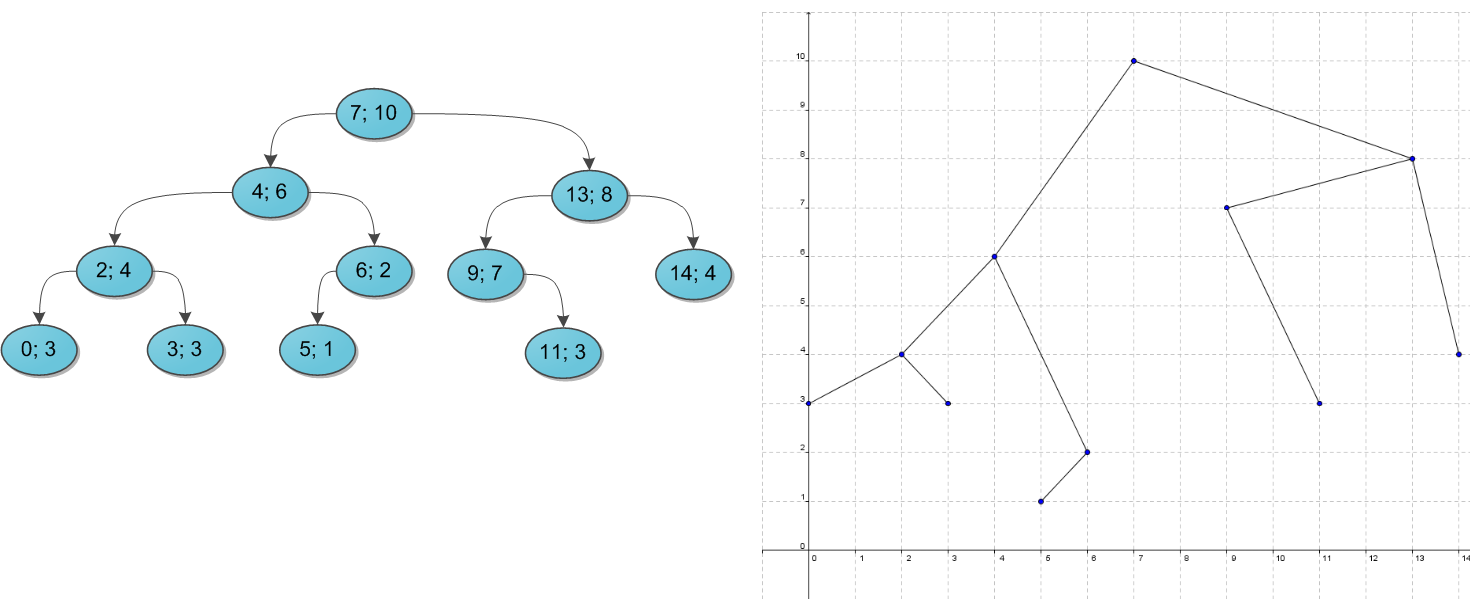
\includegraphics[width=1\linewidth]{decart.png}
    \label{decart}
\end{center}
\begin{center}
    \textit{Одно и то же дерево в обычном представлении и в виде декартового дерева}
\end{center}
При добавлении второго ключа $y$ представление дерева становится однозначным\\[2mm]
Например, правым сыном корня будет самая верхняя вершина, находящаяся справа от корня, а левым — самая верхняя вершина слева от корня\\[2mm]
\indent\textbf{Сложность} — $O(\log N)$, так как координаты $y$ выбираются случайно, то дерево получается сбалансированным и его высота равна $O(\log N)$

\subsection{По неявному ключу}
Работа с ДД по неявному пригодится в случае, если есть такие операции:
\begin{enumerate}
    \item выводить сумму на произвольном отрезке
    \item «переворачивать» произвольный отрезок, то есть переставлять элементы с $l$ по $r$ в обратном порядке, не меняя остальные
\end{enumerate}
Так как во второй операции невозможно быстро поддерживать ключи актуальными, то делаем следующее:
\begin{itemize}
    \item Убираем ключи
    \item Вместе с каждой вершиной храним размер ее поддерева
    \item Ключ (позицию элемента) восстанавливаем как число элементов слева от него
    \item Размер деревьев поддерживаем с помощью вспомогателной функции, вызываемой после каждого изменения дерева:
\end{itemize}
\begin{lstlisting}
int size(Node *v) { return v ? v->size : 0; }

void upd(Node *v) { v->size = 1 + size(v->l) + size(v->r); }
\end{lstlisting}
\textbf{Сложность} — $O(\log N)$
\subsection{Операции}
Создадим структуру \code{Node}, в которой будем хранить ключ, приоритет и указатели на левого и правого сына\\[2mm]
\indent Сначала описывается реализация по явному ключу, после — по неявному
\subsubsection{Merge}
Принимает два дерева (два корня, $L$ и $R$), про которые известно, что в левом все вершины имеют меньший ключ, чем все в правом. Их нужно объединить в одно дерево так, чтобы по ключам это было всё ещё дерево, а по приоритетам — куча\\[2mm]
\indent Сначала выберем, какая вершина будет корнем. Возьмем ту, у которой приоритет больше\\[2mm]
\indent Пусть это будет левый корень. Тогда левый сын корня итогового дерева должен быть левым сыном $L$. С правым сыном сложнее: возможно, его нужно смерджить с $R$. Поэтому рекурсивно сделаем \code{merge(l->r, r)} и запишем результат в качестве правого сына
\begin{lstlisting}
Node* merge (Node *l, Node *r) {
    if (!l) return r;
    if (!r) return l;
    if (l->prior > r->prior) {
        l->r = merge(l->r, r);
        return l;
    }
    else {
        r->l = merge(l, r->l);
        return r;
    }
}
\end{lstlisting}
По неявному ключу операция не изменится, так как нигде не использует ключи

\subsubsection{Split}
Принимает дерево и ключ $x$, по которому его нужно разделить на два: $L$ должно иметь все ключи не больше $x$, а $R$ должно иметь все ключи больше $x$\\[2mm]
\indent В этой функции мы сначала решим, в каком из деревьев должен быть корень, а потом рекурсивно разделим его правую или левую половину и присоединим, куда надо:
\begin{lstlisting}
typedef pair<Node*, Node*> Pair;

Pair split (Node *p, int x) {
    if (!p) return {0, 0};
    if (p->key <= x) {
        Pair q = split(p->r, x);
        p->r = q.first;
        return {p, q.second};
    }
    else {
        Pair q = split(p->l, x);
        p->l = q.second;
        return {q.first, p};
    }
}
\end{lstlisting}
По неявному ключу операция немного изменяется. Теперь нужно использовать позицию корня вместо ключа. \code{Split} теперь выполняет такую команду, как «вырежи первые $k$ элементов»
\begin{lstlisting}
pair<Node*, Node*> split(Node *p, int k) {
    if (!p) return {0, 0};
    if (size(p->l) + 1 <= k) {
        auto [l, r] = split(p->r, k - size(p->l) - 1);
        p->r = l;
        upd(p);
        return {p, r};
    }
    else {
        auto [l, r] = split(p->l, k);
        p->l = r;
        upd(p);
        return {l, p};
    }
}
\end{lstlisting}

\subsection{Применение декартового дерева}
Операции \code{Merge} и \code{Split} позволяют реализовать следующие операции
\subsubsection{Вставка}
Например, чтобы добавить число $x$ в дерево, мы можем разрезать его по $x$ через \code{split}, создать новую вершину с одним числом $x$, и склеить через \code{merge} три получившихся дерева

\subsubsection{Сумма на отрезке}
% Для этого в вершине нужно хранить также своё число и сумму на своем «отрезке»
\begin{itemize}
    \item При \code{merge} и \code{split} надо будет поддерживать эту сумму актуальной
    \item Можно написать вспомогательную функцию \code{upd}, которую будем вызывать при обновлении детей вершины
    \item В \code{merge} и \code{split} теперь можно просто вызывать \code{upd} перед тем, как вернуть вершину
    \item При запросе суммы нужно вырезать нужный отрезок и запросить эту сумму
\end{itemize}

\subsubsection{Переворот}
Добавим флаг \code{rev} в каждую вершину, означающий, что подотрезок был перевернут\\[2mm]
\indent Когда мы встретим такую вершину, мы поменяем местами ссылки на её детей, а им самим передадим эту метку\\[2mm]
\indent Тогда функция \code{reverse} будет такой: вырезаем нужный отрезок, меняем флаг


\end{document}
